%!TEX root = paper.tex
\subsection{Skimmers in the wild} %{{{
\label{sec:skimmersinwild}

\begin{table}
    \centering\small
    \begin{tabular}{lrrrr}
\toprule
\colname{Parameter} & \colname{2016} & \colname{2017} & \colname{2018} & \colname{All} \\
\midrule
\textbf{Routine Inspections} \\
\quad Total & 2,116 & 928 & 1,311 & 4,355 \\
\quad Found skimmers & 28 & 30 & 45 & 103 \\
\emph{Effectiveness} & 1.3\% & 3.2\% & 3.4\% & 2.4\% \\
\hline
\textbf{Complaint Inspections} \\
\quad Total & 53 & 63 & 128 & 244 \\
\quad Found skimmers & 3 & 5 & 12 & 20 \\
\emph{Effectiveness} & 5.7\% & 7.9\% & 9.3\% & 8.2\% \\

%Effectiveness of  & 2,116 & 928 & 1,311 & 4,355 \\
%Inspections triggered by Complaints & 53 & 63 & 128 & 244 \\
%Inspections recovering Skimmers & 28 & 27 & 38 & 93 \\
%Percent Skimmer Complaint Hits & 0 & 0 & 0 & 0 \\
%Percent Skimmer Investigation Hits & 0 & 0 & 0 & 0 \\
%(\%) Complaint-based Inspection Hits & \\
%\quad Avg. days since last insp. & 175.7 & 129.3 & 120.2 & 136.7 \\
%Skimmed stations & \azXVIsksta & \azXVIIsksta & \azXVIIIsksta & \azALLsksta \\
%\quad Gilbarco Advantage & \azXVIadvantage & \azXVIIadvantage & \azXVIIIadvantage & \azALLadvantage \\
%\quad Gilbarco Encore 300 & \azXVIencoreIII & \azXVIIencoreIII & \azXVIIIencoreIII & \azALLencoreIII \\
%\quad Gilbarco Encore 500s & \azXVIencoreV & \azXVIIencoreV & \azXVIIIencoreV & \azALLencoreV \\
%\quad Wayne Vista & \azXVIvista & \azXVIIvista & \azXVIIIvista & \azALLvista \\
%\quad Wayne Ovation & \azXVIovation & \azXVIIovation & \azXVIIIovation & \azALLovation \\
%Station risk  & \azXVIstarisk & \azXVIIstarisk & \azXVIIIstarisk & \azALLstarisk \\
%Skimmers recovered & \azXVIskimmers & \azXVIIskimmers & \azXVIIIskimmers & \azALLskimmers \\
%\quad Streetside & \azXVIstreet & \azXVIIstreet & \azXVIIIstreet & \azALLstreet \\
%\quad Storeside & \azXVIstore & \azXVIIstore & \azXVIIIstore & \azALLstore \\
%Sk. per incident & \azXVIskperinc & \azXVIIskperinc & \azXVIIIskperinc & \azALLskperinc \\
\bottomrule
\end{tabular}
    \caption{Routine inspections routinely do not find skimmers, but complaint-triggered inspections are significantly
    more likely to find skimmers.}
    \label{tab:azwm-results}
\end{table}

In previous subsections, we have identified the monetary cost of every single skimmer recovered in the field. In this subsection, we use data available from skimmer-hotbed areas of Arizona state and San Diego region to understand the prevalence of this problem. Armed with this understanding of gas station vulnerabilities in these regions that enable this problem, we perform a Google Street View based nationwide sampling of gas stations, to identify the potential prevalence of this threat across the US. Finally we close off by analyzing Arizona data further to understand effectiveness of current manual inspection methods and skimmer complaint mechanisms in Arizona. This motivates the need to augment existing investigative techniques with new pieces of information for improving the status quo.

\subsubsection*{Dataset Overview}

The Southwest of the U.S. is an area of elevated skimmer activity, leading us to focus on these two parts of the U.S.

The Arizona Department of Weights and Measures (AZWM) is tasked, among other responsibilities, with inspecting fuel dispensers for compliance with Arizona state laws and regulations. While the purpose of most inspections is not to search for skimmers, if inspectors do a find skimmers, they report this on the Fueling Device Inspection Form. AZWM makes all inspections reports available publicly in PDF form on their Web site.\footnote{\url{https://ctutools.azda.gov/PdfOriginals/}} The form includes the following data items: gas station street address, inspection date, time spent on the inspection, description of the complaint if inspection is based on a complaint, the last 5 inspections done at same location with date, and a description of the current inspection. If a skimmer is found, this is noted on the Fueling Device Inspection Form, and, in some cases, is accompanied by a Skimmer Inspection Form.

We downloaded all AZWM inspection reports and extracted all Fueling Device Inspection Form data and Skimmer Inspection Form data for analysis. Table~\ref{tab:azwm-results} summarizes our results.

\subsubsection{Prevalence of skimmers} %{{{

\paragraph{Arizona} \noteby{AS}{Nishant needs to write the rest of this text} \azALLskimmers~skimmers were
Recovered at skimmed stations, which amounts to \azALLskperinc~per incident.
While the number of skimmers are low, in section~\ref{subsec:skimcost} we show that the losses are huge

\paragraph{San Diego and Imperial counties} The San Diego office of the United States Secret Service is responsible
for San Diego and Imperial counties, which span the California--Mexico border. Unlike the AZWM, the USSS does not
routinely inspect fuel dispensers; all inspections are triggered by reports of a skimmer or a pattern of credit card
fraud that suggests a skimmer may be present at a fuel station.

%\begin{table}
%    \centering
%    \begin{tabular}{lr}
\toprule
\colname{Parameter} & \colname{FY18} \\
\midrule
% Inspections & XXX \\
Incidents & \usssfyXVIIIincidents \\
% Insp. hit rate & XXX \\
Sk. stations & \usssfyXVIIIsksta \\
Station risk & \usssfyXVIIIstarisk \\
Skimmers & \usssfyXVIIIskimmers \\
Sk. per incident & \usssfyXVIIIskperinc \\
\bottomrule
\end{tabular}
%    \caption{Summary of skimmer recovery statistics from the San Diego office of the United States Secret Service.}
%    \label{tab:usss-results}
%\end{table}

We obtained skimmer recovery statistics from the San Diego office of the United
States Secret Service for the 12 month period from October 1, 2017 to September
30, 2018. Table~\ref{tab:usss-results} summarizes these statistics.
\noteby{KL}{Discuss USSS results.}
\begin{comment}
\begin{figure}
    \centering
    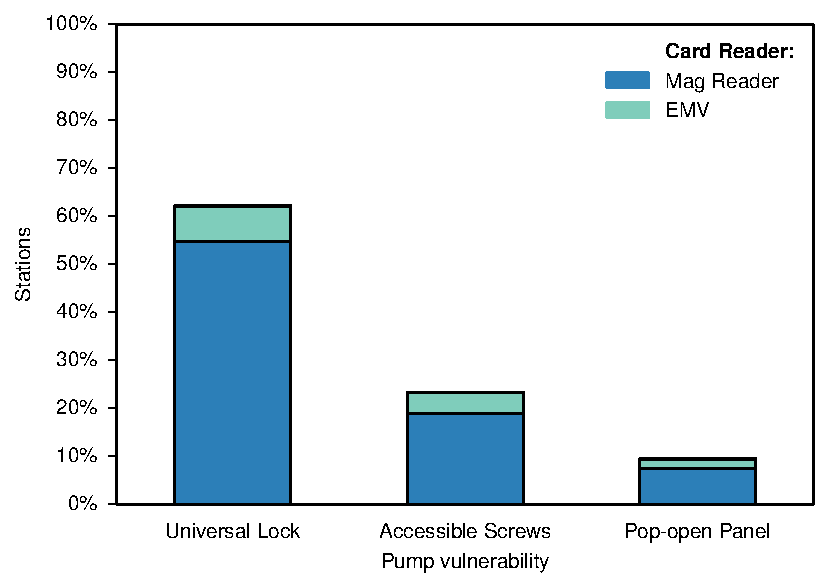
\includegraphics[width=\linewidth]{plots/barplot_us_vul_list.pdf}
    \caption{
    \label{fig:cdf_usvulgasstation}
    More than 80\% of gas stations across US, are still using easily accessible dispensers with magnetic card readers
    }
\end{figure}
\end{comment}
\paragraph{Nationwide prevalence of vulnerable pumps}
%

From the Arizona dataset we also know the make and model of gas dispensers on which skimmers were recovered. Gilbarco dispensers accounted for 84.8\% of skimmed stations with the numbers split between different models - Advantage (30.6\%), Encore 500s (36.6\%) and Encore 300 (17.6\%). Wayne dispensers accounted for 15.2\%. Since skimmers were discovered on these particular dispensers, a natural question arises - how common are these dispensers nationwide?

To answer this question, we performed a nationwide survey of gas stations across the US, with the aim of figuring out how prevalent are these particular dispensers. To identify the particular dispenser in service at a gas station, we can use Google Street View images, which surprisingly have a decent resolution for our task. We grouped all the gas stations across the US into population-served brackets using public FIPS data of the specific areas where the gas stations are located. The goal of population binning is to cover a wide variety of urban to semi-urban areas. In the top three population brackets - population in order of millions, order of hundreds of thousands and
order of tens of thousands, we randomly selected 0.5\% of all gas stations. For each of the gas stations selected, we manually inspected the Google Street View images to identify make and model of the dispenser. Additionally, since we know that there has been a push to retrofit these particular dispensers with EMV readers to remove the magnetic reader vulnerability, we identify the card reader with tha aim of understanding how widespread the use of EMV is. 

\begin{comment}
model and card reader type of dispensers. All the gas stations across the US
were divided into population-served brackets using public FIPS data of the
specific areas where the gas stations are located. In the top three population
brackets - population in order of millions, order of hundreds of thousands and
order of tens of thousands, we randomly selected 0.5\% of all gas stations, and
used Street View images to identify how many of these gas stations had
dispensers that suffered from three known vulnerabilites - use of a universal
lock, easily accessible door screws and pop-open card reader access.
Figure~\ref{fig:cdf_usvulgasstation} demonstrates the results.
\end{comment}
From the analysis, we observed that Gilbarco dispensers - Advantage, Encore 300 and Encore 500s are still the most popular across the country with 62.26\% of all dispensers sampled. Wayne Ovation and Vista account for another 32.79\%. The newer and secure models like Wayne Helix and Encore 700s currently only account for 1.61\% of all dispensers in the sample set, revealing the status quo of migration to secure dispensers. Even retrofitting to EMV had significantly low adoption. Of the 62.26\% of Gilbarco dispensers, only 7.44\% had EMV, and for Wayne this number stands at 6.43 \%. From these numbers, it can clearly be seen that the problem of skimmer vulnerable dispensers is significant all across the nation.

%}}}

\subsubsection{Effectiveness of inspections and complaints} %{{{

Analysis of Arizona inspection data reveals the challenges faced with the
status quo for skimmer discovery. While skimmer inspections comprised
\azALLskinsppct~of all inspections in the period from 2016-2018, skimmers were
recovered in only \azALLinsphr~of these. Skimmer complaints, often perceived to
be a viable source of skimming information, are surprisingly ineffective. Only
\azALLskinc~of successful skimmer inspections were due to a skimming complaint.
Worse still, of all the skimmer complaints only \azALLskinsphr~resulted in a
hit, revealing that these reports are also very unreliable. In this period,
skimmers were recovered at only \azALLsksta~gas stations, which meant that if
investigators were to randomly inspect an Arizona station, they only had a
\azALLstarisk chance of finding a skimmer. The year-by-year
breakdowns follow similar trends as the overall numbers. Interestingly though,
while the year 2018 saw a drop in ratio of skimmer
inspections~(\azXVIIIskinsppct)~over previous years, we observe a significant
increase in the number of incidents~(\azXVIIIincidents),~inspection hit
rate~(\azXVIIIinsphr)~and also number of skimmers
recovered~(\azXVIIIskimmers).~This is a result of increased knowledge among
consumers, station owners and the inspectors about skimmers. While this has
improved the effectivenss of skimmer inspections, still leaves a lot to be
desired.

\begin{figure}
    \centering
    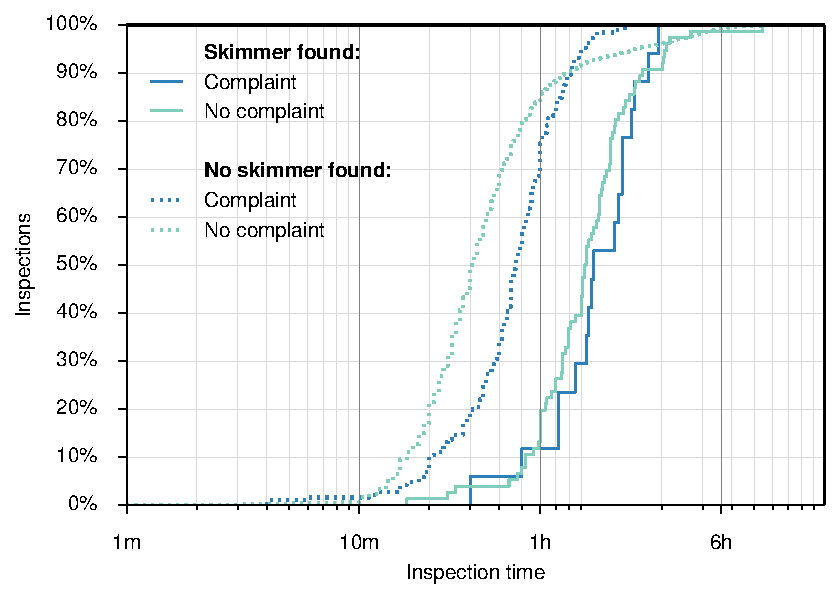
\includegraphics[width=\linewidth]{plots/arizona_analysis_all.pdf}
    \caption{
    \label{fig:cdf_arizona_timetaken}
    50\% of the unsuccessful manual inspections for skimmers took over half an hour to complete
    }
\end{figure}

But how costly in time is an inspection for Weights and Measures? All
inspection reports mention a start and end time for the inspection, and we use
that to analyze the time taken per inspection. Figure
\ref{fig:cdf_arizona_timetaken} shows the distribution of durations for
inspections that found skimmers and inspections that did not, split up by
whether inspection was triggered by a skimming complaint or not.

From the figure it can be observed that more time is spent in an inspection
when a skimmer was discovered. This is expected as the skimmer needs to be
carefully removed, tagged and bagged for forensic evidence. Also inspection
triggered by complaints take more time than their regular inspection
equivalents, which is also expected as a complaints need to be investigated
thoroughly. The interesting piece of information is the median time of
inspections. The median time for an unsuccessful inspection is 30 min (regular
inspection) and almost 50 min (complaint). From table~\ref{tab:azwm-results},
we know the number of unsuccessful inspections, and therefore the total time
spent by inspectors in unsuccessful inspections is 2,312 human-hours, or about
14 months(40 hours/week) of full time labor.Note that this is a conservative
estimate because it does not include transportation time, only the time spent
opening and searching fuel dispensers. Given limited agency resources, a
skimmer may be in place for months before it is found by a random inspection.
For 2018, we calculated the number of days to a successful skimmer recovery from a previous inspection at that same location and it turns out to be 120 days, which can result in significant monetary fraud.
%}}}

%}}}
